\begin{theorem}
    Suppose we have a function $f \in \operatorname{C}^1([a, b])$, such that:
    \begin{enumerate}
        \item {
            $f(a) \cdot f(b) < 0$ (there's a sign switch).
        }
        \item {
            $f'$ has no critical points in $(a, b)$.
        }
        \item {
            $f''$ exists, is continuous and either $f'' > 0$
            or $f'' < 0$ in $(a, b)$.
            I.e., $f$ is either concave down or concave up.
        }
    \end{enumerate}
    Then $f(x) = 0$ has \textit{exactly one} solution $r$. 
    The Newton sequence always converges to $r$.

    For $n \to \infty$, when the initial guess should be chosen according to:
    \begin{itemize}
        \item {
            If $f(a) < 0$, $f'' < 0$ or $f(a) > 0, f'' > 0$
            then $x_0 \in [a, r]$, e.g. $x_0 = a$.
        }
        \item {
            If $f(a) < 0$, $f'' > 0$ or $f(a) > 0$, $f'' < 0$ then
            $x_0 \in [r, b]$, e.g. $x_0 = b$.
        }
    \end{itemize}
    (If we chose an initial guess on the wrong side of the graph, then 
    the Newton method may diverge outside the domain area of  $(a, b)$ --- we don't want that.)

    In any case we have the estimate
    \[ \abs{x_n - r} < \frac{f(x_n)}{\min_{[a, b]} \abs{f'(x)}} \]
\end{theorem}

Problems with the Newton method:
\begin{enumerate}
    \item {
        The runaway problem: the Newton method may start stepping in the wrong side.
        \begin{figure*}[h]
            \centering
            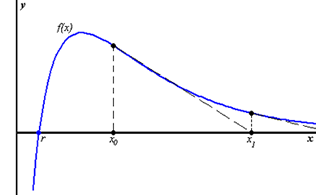
\includegraphics[width=0.5\textwidth]{runaway}
        \end{figure*}
    }
    \item {
        If we have a flat point, we don't know in which direction to go:
        \begin{figure*}[h]
            \centering
            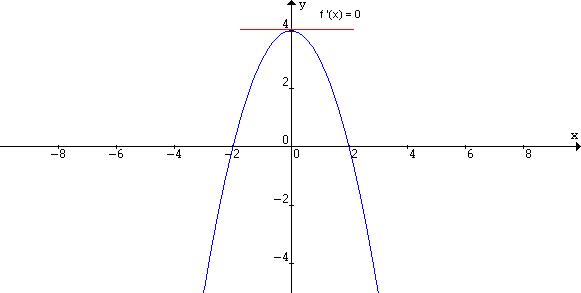
\includegraphics[width=0.5\textwidth]{flat_point}
        \end{figure*}
    }
    \item {
        Sometimes the Newton method can jump infinitely between two points in a cycle
        without ever converging.
        \begin{figure*}[h]
            \centering
            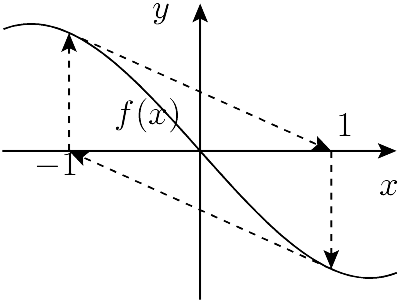
\includegraphics[width=0.5\textwidth]{newton_cycle}
        \end{figure*}
    }
\end{enumerate}
\pagebreak
\begin{theorem}
    If $f : [a, b] \to \mathbb{R}$ fullfills:
    \begin{enumerate}
        \item {
            $f(a) \cdot f(b) < 0$.
        }
        \item {
            $f$ has no critical points in $(a, b)$.
        }
        \item {
            $f''$ exists and is continuous ($f \in \operatorname{C}^2([a, b])$)
            and $x_0$ needs to \textit{``close enough''} (not a mathematical term)
            to the root $r$.
        }
    \end{enumerate}
    Then the Newton sequence converges quadratically.
\end{theorem}
\begin{proof}
    We have to show that
    $\abs{x_{n + 1} - r} \le M \abs{x_n - r}^2$ as $n \to \infty$.
    By Taylor series approximation,
    \[ 
        f(x) = f(x_n) + f'(x_n)(x - x_n) + \frac{1}{2} f''(\xi_n)(x - x_n)^2 
        \text{, where } \xi_n \in (x, x_n)
    \]
    Since $r$ is a root of $f$, when we put $x = r$, we get
    \[
        0 = f(r) = f(x_n) + f'(x_n)(r - x_n) + \frac{1}{2} f''(\xi_n)(r - x_n)^2
    \]
    Let's divide both sides by $f'(x_n)$ and rearrange the terms:
    \begin{align*}
        &\frac{f(x_n)}{f'(x_n)} +
        \frac{f'(x_n)}{f'(x_n)} (r - x_n) = -\frac{f''(\xi_n)}{2 f'(x_n)}(r-x_n)^2
        \\&\Longleftrightarrow (r - x_{n+1}) = -\frac{f''(\xi_n)}{2 f'(x_n)} (r - x_n)^2
        \quad \Bigl(x_{n+1} = x_n - \frac{f(x_n)}{f'(x_n)}\Bigr)
        \\&\implies \abs{r - x_{n+1}} = \abs{\frac{f''(\xi_n)}{2f'(x_n)}} \abs{r - x_n}^2
    \end{align*}
    Let
    \[ M \coloneqq \sup_{x_n,\, \xi_n} \abs{\frac{f''(\xi_n)}{2f'(x_n)}} \]
    The supremum will be finite, because $x_n$ and $\xi_n$ are both
    inside bounded intervals.

    Then $\abs{r - x_{n + 1}} \le M \abs{r - x_n}^2$.
\end{proof}
\begin{remark}
    We need $x_0$ to be close enough to make sure the Newton method
    doesn't go outside the domain $[a, b]$.
\end{remark}

\subsection{Modifications of the Newton method}
\subsubsection{Modified Newton method}
As we remember, in the usual Newton method
\[ x_{n+1} = x_n - \frac{f(x_n)}{f'(x_n)} \]
If $f'(x_n)$ doesn't change much anymore from $n$ to $n + 1$, we can fix it to
$f'(x_m)$ with some fixed $m \le n$. Then our new formula for $x_{n+1}$ is
\[ x_{n + 1} = x_n - \frac{f(x_n)}{f'(x_m)} \]
We avoid futher evaluations of $f'(x)$ which saves computational resources.

\subsubsection{Secant method}
Newton's method needs derivatives. 
We can approximate the derivatives by secants (also called a difference quotient):

\[
    f'(x) = \lim_{h \to 0} \frac{f(x + h) - f(x)}{h} \implies
    f'(x) \approx \frac{f(x + h) - f(x)}{h} \text{ for small $h$}
\]
For the Secant method, we let $x_n \coloneqq x_n,\ h \coloneqq x_{n - 1} - x_{n}$.
\[ f'(x_n) \approx \frac{f(x_{n - 1}) - f(x_n)}{x_{n - 1} - x_{n}} \]
Substitution into Newton method gives us
\[ x_{n + 1} = x_{n} - \frac{f(x_n) (x_{n - 1} - x_{n})}{f(x_{n - 1}) - f(x)} \]

The Secant method converges slower than the Newton method, but it's easier to compute.

\begin{theorem}
    If $f \in \operatorname{C}^2([a, b])$
    and $r \in (a, b),\ f(r) = 0,\ f'(r) \ne 0$
    and 
    \[ x_{n + 1} = x_n - \frac{f(x_n) (x_{n-1} - x_n)}{f(x_{n - 1} - f(x_n))} \]
    Then there exists a $\delta > 0$, such that for every $x_1, x_0$, such that
    $\abs{r - x_1} < \delta$, $\abs{r - x_0} < \delta$, we'll have
    \begin{enumerate}
        \item {
            $\lim_{n \to \infty} \abs{x_n - r} = 0$ (the sequence converge)
        }
        \item {
            $\abs{r - x_{n + 1}} \le M \abs{r - x_n}^\alpha$
            with $\alpha = \frac{1 + \sqrt{5}}{2} \approx 1.618$
            (the sequence converges with order of golden ratio).
        }
    \end{enumerate}
\end{theorem}
\begin{example}
    \[ f(x) = x^5 - 3x + 1 = 0,\ f'(x) = 5x^4 + 3 \]
    Newton method:
    \begin{align*}
        &x_0 = 0,\ f(0) = 1,\ f'(0) = 3
        \\&
        x_1 = x_0 = \frac{f(x_0)}{f'(x_0)} = 0 - \frac{1}{3} = -\frac{1}{3}
    \end{align*}

    Secant method:
    \begin{align*}
        &x_0 = 1,\ x_1 = \frac{1}{2}
        \\&
        x_2 = \frac{1}{2} - \frac{f(1/2)(1 - 1/2)}{f(1) - f(1/2)} = \dots
    \end{align*}
\end{example}

Summary:
{
\tiny
\[\begin{array}{c|c|c|c|c|c}
    & \text{\#initials} & \text{Regularity of $f$} & \text{Convergence} & \text{Root between points} & \text{Function calls per iteration}
    \\\hline
    \text{Bisection} & \text{2 ($a$, $b$)} & \operatorname{C}([a, b]) & \text{linear} & \text{Yes} & 1
    \\\hline
    \text{Newton} & \text{1 ($x_0$)} & \operatorname{C^2}([a, b]) &
    \text{quadratic} & \text{No} & 2
    \\\hline
    \text{Secant} & \text{2 ($x_0$, $x_1$)} & \operatorname{C^2}([a, b]) &
    \text{superlinear/order $\alpha = 1.618$} & \text{No} & 1
\end{array}
\]
}